\section{Casi d'uso}

\subsection{Introduzione}
All'interno di questa sezione vengono elencati i casi d'uso rilevanti per il prodotto
MegAlexa individuati e definiti attraverso l'analisi del \glo{capitolato} d'appalto,
gli incontri con il proponente e le riunioni interne al team \groupName{}.
Ogni caso d'uso rappresenta un insieme di scenari che hanno in comune uno scopo finale per un utente generico del sistema, chiamato \glo{attore}.
La struttura e le convenzioni usate in ogni caso d'uso sono specificate all'interno del documento \docNameVersionNdP{}.

\subsection{Codice identificativo}
Ogni caso d'uso è classificato secondo la seguente sintassi:

\begin{center}
\textbf{UC \{XX\} . \{YY\}}
\end{center}

dove:

\begin{itemize}
    \item \textbf{UC:} Use Case;
    \item \textbf{{XX}:} numero che identifica i casi d'uso;
    \item \textbf{{YY}:} numero progressivo che identifica i sotto casi, esso può, a sua volta, includere altri sotto casi.
\end{itemize}


\subsection{Interfaccia}
Le interfacce sviluppate saranno organizzate nei seguenti aspetti:
\begin{itemize}
    \item \textbf{Interfaccia Mobile}: descrizione nell'applicazione \glo{Android} di come verrà sviluppata.
\end{itemize}

\subsection{Attori dei casi d'uso}
\begin{itemize}
    \item \textbf{Attori primari}: 
    
    \begin{enumerate}
    \item \textbf{Utente non autenticato}: si riferisce all'utente che non ha ancora eseguito il login al sistema;
     \item \textbf{Utente autenticato}: si riferisce all'utente che ha effettuato il login al sistema.
\end{enumerate}    
    
    \item \textbf{Attori secondari}:
    \begin{enumerate}
    \item \textbf{Amazon};
    \item \textbf{Instagram};
    \item \textbf{Facebook};
    \item \textbf{LinkedIn};
    \item \textbf{Slack};
    \item \textbf{Telegram};
    \item \textbf{Google}.
    \end{enumerate}
\end{itemize}
\pagebreak
\subsection{Elenco dei casi d'uso}


\subsubsection{Visione ad alto livello - Utente non autenticato}

\begin{figure}[H]
\centering
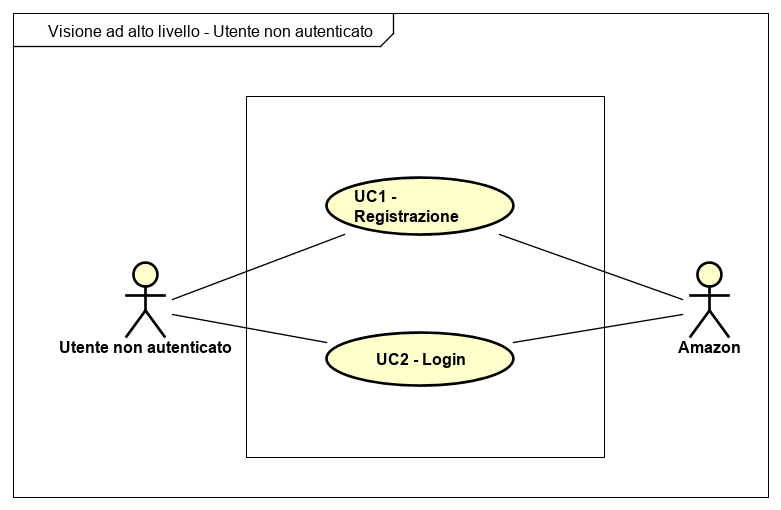
\includegraphics[scale=0.7]{immagini/UC0-1.png}
\caption{Visione ad alto livello - Utente non autenticato \label{fig:uc0-1}}
\end{figure}
\begin{itemize}
\item \textbf{Attori primari}: utente non autenticato;

\item \textbf{Attori secondari}: Amazon;

\item \textbf{Descrizione}: se l'attore non ha un account, può registrarsi al sistema tramite account Amazon, altrimenti può fare il login;

\item \textbf{Pre-condizione}: l'attore si trova nella homepage dell'applicazione;

\item \textbf{Post-condizione}: l'attore è loggato nel sistema e si trova nella homepage dell'applicazione;

\item \textbf{Scenario principale}:
\begin{enumerate}
\item l'utente può registrarsi al sistema (UC1);
\item l'utente può loggarsi al sistema (UC2).
\end{enumerate}

\end{itemize}
\pagebreak
\subsubsection{Visione ad alto livello - Utente autenticato}
\begin{figure}[H]
\centering
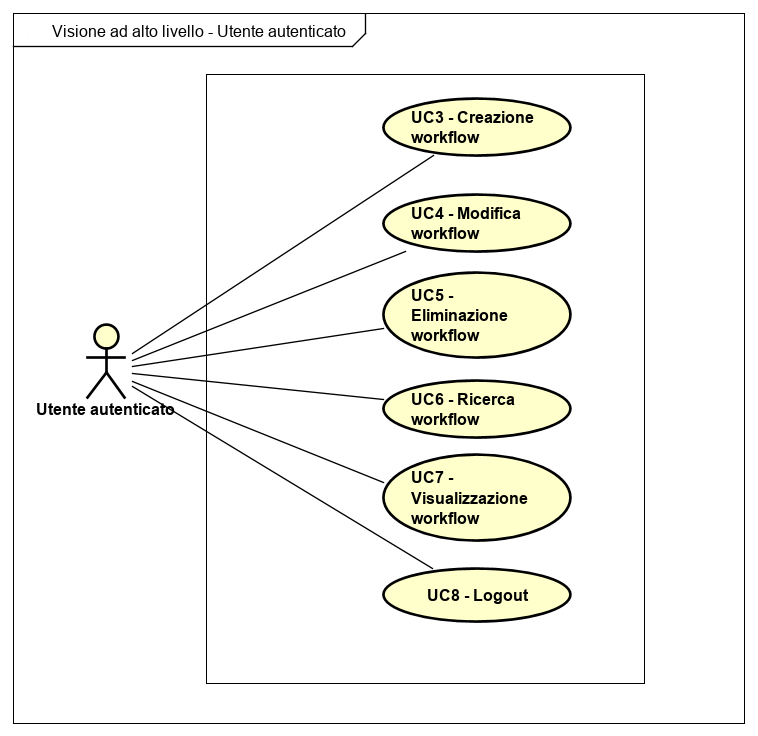
\includegraphics[scale=0.7]{immagini/UC0-2.png}
\caption{Visione ad alto livello - Utente autenticato \label{fig:uc0-2}}
\end{figure}

\begin{itemize}
\item \textbf{Attori primari}: utente autenticato;

\item \textbf{Descrizione}: l'attore può accedere alle funzionalità dell'applicazione;

\item \textbf{Pre-condizione}: l'attore deve essere correttamente autenticato al sistema;

\item \textbf{Post-condizione}: il sistema esegue correttamente le funzionalità;

\item \textbf{Scenario principale}:
\begin{enumerate}
\item l'utente può creare un workflow (UC3);
\item l'utente può modificare un workflow (UC4);
\item l'utente può eliminare un workflow (UC5);
\item l'utente può ricercare un workflow (UC6);
\item l'utente può visualizzare i workflow creati (UC7);
\item l'utente può effettuare il logout (UC8).

\end{enumerate}

\end{itemize}

\subsubsection{UC1 - Registrazione}

\begin{itemize}
\item \textbf{Attori primari}: utente non autenticato;

\item \textbf{Descrizione}: per accedere all'applicazione è necessario che l'attore si registri ad Amazon;

\item \textbf{Pre-condizione}: l'attore non possiede un account Amazon;

\item \textbf{Post-condizione}: è stato creato un account Amazon per accedere all'applicazione;

\item \textbf{Scenario principale}:
\begin{enumerate}
\item l'utente clicca sul pulsante per la registrazione;
\item l'utente viene reindirizzato alla pagina di registrazione di Amazon;
\item l'utente completa la registrazione;
\item l'utente viene reindirizzato all'homepage dell'applicazione.

\end{enumerate}

\end{itemize}

\subsubsection{UC2 - Login}

\begin{itemize}
\item \textbf{Attori primari}: utente non autenticato;

\item \textbf{Attori secondari}: Amazon;

\item \textbf{Descrizione}: per utilizzare l'applicazione l'attore deve essere autenticato;

\item \textbf{Pre-condizione}: l'attore possiede un account Amazon e vuole autenticarsi nel sistema;

\item \textbf{Post-condizione}: l'attore è autenticato nel sistema;

\item \textbf{Scenario principale}:
\begin{enumerate}
\item l'utente preme sul pulsante per accedere al sistema;
\item viene reindirizzato alla pagina di login di Amazon;
\item l'utente conferma le credenziali di accesso;
\item l'utente viene reindirizzato alla homepage dell'applicazione.

\end{enumerate}

\end{itemize}
\pagebreak
\subsubsection{UC3 - Creazione workflow}

\begin{figure}[H]
\centering
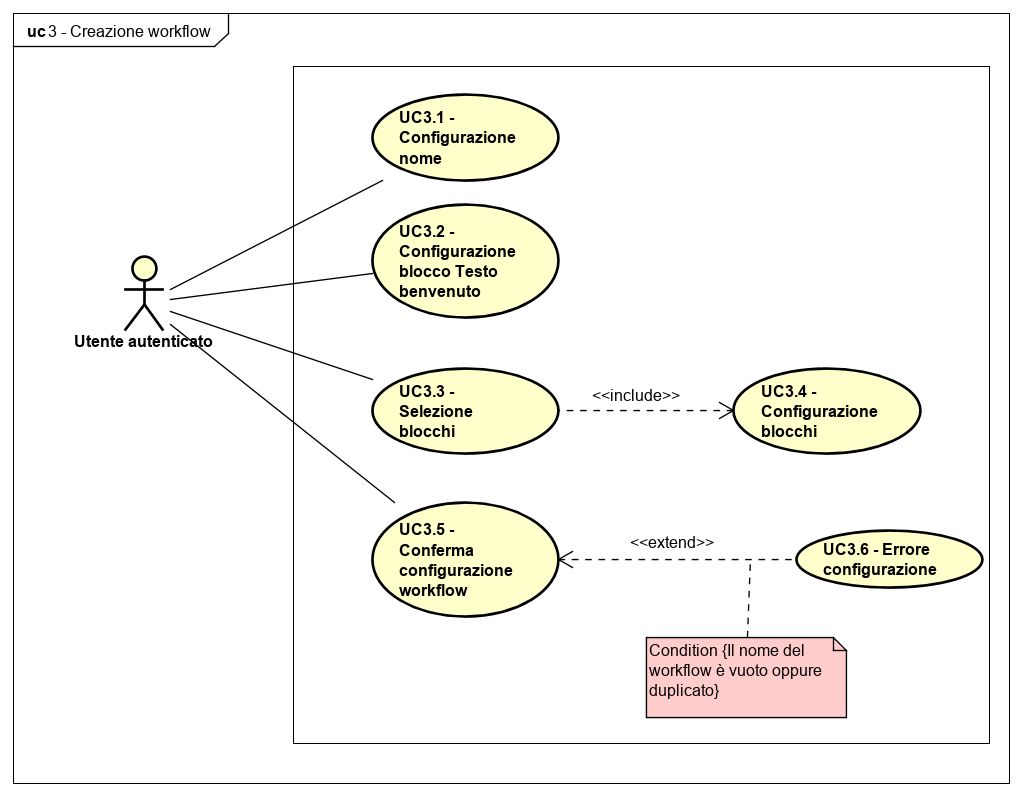
\includegraphics[scale=0.6]{immagini/UC3}
\caption{UC3 - Creazione workflow \label{fig:UC3}}
\end{figure}

\begin{itemize}
\item \textbf{Attori primari}: utente autenticato;

\item \textbf{Descrizione}: l'attore può creare un workflow personale scegliendo e configurando i blocchi tra quelli disponibili;

\item \textbf{Pre-condizione}: l'attore vuole creare un nuovo workflow;

\item \textbf{Post-condizione}: il workflow è stato creato e i dati sono inseriti nel sistema;

\item \textbf{Scenario principale}:
\begin{enumerate}
\item l'utente può dare un nome al workflow (UC3.1);
\item l'utente può configurare il \BBenvenuto{} (UC3.2);
\item l'utente può selezionare i blocchi da inserire all'interno del workflow (UC3.3);
\item l'utente conferma la configurazione del workflow (UC3.5).

\end{enumerate}
\item \textbf{Inclusione}: l'utente può configurare i blocchi selezionati (UC3.4);
\item \textbf{Estensione}: viene visualizzato un errore a video se i dati sono sbagliati (UC3.6).
\end{itemize}

\pagebreak
\item \textbf{Diagramma delle attività}
\begin{figure}[H]
\centering
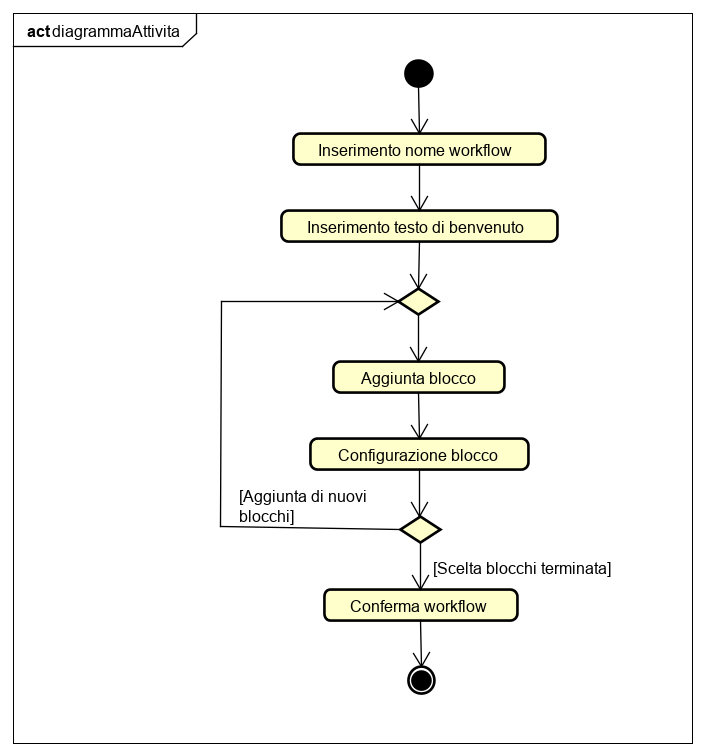
\includegraphics[scale=0.7]{immagini/diagrammaAttivita}
\caption{Diagramma delle attività per creazione workflow \label{fig:diagrammaAttivita}}
\end{figure}

\paragraph{UC3.1 - Configurazione nome}

\begin{itemize}
\item \textbf{Attori primari}:  utente autenticato;

\item \textbf{Descrizione}: l'attore può dare un nome al workflow;

\item \textbf{Pre-condizione}: il workflow non ha ancora un nome;

\item \textbf{Post-condizione}: il workflow ha un nome univoco dato dall'utente;

\item \textbf{Scenario principale}:
\begin{enumerate}
\item l'utente può inserire il nome del workflow.

\end{enumerate}
\end{itemize}

\paragraph{UC3.2 - Configurazione blocco testo benvenuto}

\begin{itemize}
\item \textbf{Attori primari}:  utente autenticato;

\item \textbf{Descrizione}: l'attore può inserire un testo di benvenuto al workflow nel blocco di testo apposito;

\item \textbf{Pre-condizione}: il \BBenvenuto{} non è ancora stato configurato;

\item \textbf{Post-condizione}: l'utente ha configurato il \BBenvenuto{};

\item \textbf{Scenario principale}:
\begin{enumerate}
\item l'utente può configurare il blocco di testo.
\end{enumerate}
\end{itemize}

\pagebreak
\paragraph{UC3.3 - Selezione blocchi}

\begin{itemize}
\item \textbf{Attori primari}: utente autenticato;

\item \textbf{Descrizione}: l'attore può selezionare i blocchi da inserire nel workflow;

\item \textbf{Pre-condizione}: l'attore vuole inserire un blocco all'interno del workflow;

\item \textbf{Post-condizione}: il blocco selezionato è pronto per essere configurato;

\item \textbf{Scenario principale}:
\begin{enumerate}
\item l'utente può scegliere di inserire il \BTesto{} nel workflow (UC3.3.1);
\item l'utente può scegliere di inserire il \BFiltro{} nel workflow (UC3.3.2);
\item l'utente può scegliere di inserire il \BFeedRSS{} nel workflow (UC3.3.3);
\item l'utente può scegliere di inserire il \BMeteo{} nel workflow (UC3.3.4);
\item l'utente può scegliere di inserire il \BInstagram{} nel workflow (UC3.3.5);
\item l'utente può scegliere di inserire il \BFacebook{} nel workflow (UC3.3.6);
\item l'utente può scegliere di inserire il \BMessenger{} nel workflow (UC3.3.7);
\item l'utente può scegliere di inserire il \BLinkedIn{} nel workflow (UC3.3.8);
\item l'utente può scegliere di inserire il \BSveglia{} nel workflow (UC3.3.9);
\item l'utente può scegliere di inserire il \BSlack{} nel workflow (UC3.3.10);
\item l'utente può scegliere di inserire il \BTelegram{} nel workflow (UC3.3.11);
\item l'utente può scegliere di inserire il \BMail{} nel workflow (UC3.3.12);
\item l'utente può scegliere di inserire il \BCalendario{} nel workflow (UC3.3.13);
\item l'utente può scegliere di inserire il \BYouTube{} nel workflow (UC3.3.14);
\item l'utente può scegliere di inserire il \BYouTubeMusic{} nel workflow (UC3.3.15);
\item l'utente può scegliere di inserire il \BRadio{} nel workflow (UC3.3.16);
\item l'utente può scegliere di inserire il \BTV{} nel workflow (UC3.3.17);
\item l'utente può scegliere di inserire il \BSpotify{} nel workflow (UC3.3.18);
\item l'utente può scegliere di inserire il \BCinema{} nel workflow (UC3.3.19);
\item l'utente può scegliere di inserire il \BTrasporti{} nel workflow (UC3.3.20);
\item l'utente può scegliere di inserire il \BLista{} nel workflow (UC3.3.21);
\item l'utente può scegliere di inserire il \BSicurezza{} nel workflow (UC3.3.22);
\item l'utente può scegliere di inserire il \BKindle{} nel workflow (UC3.3.23).

\end{enumerate}
\item \textbf{Inclusione}: l'utente può configurare i blocchi selezionati (UC3.4).
\end{itemize}

\begin{figure}[htbp]
\centering
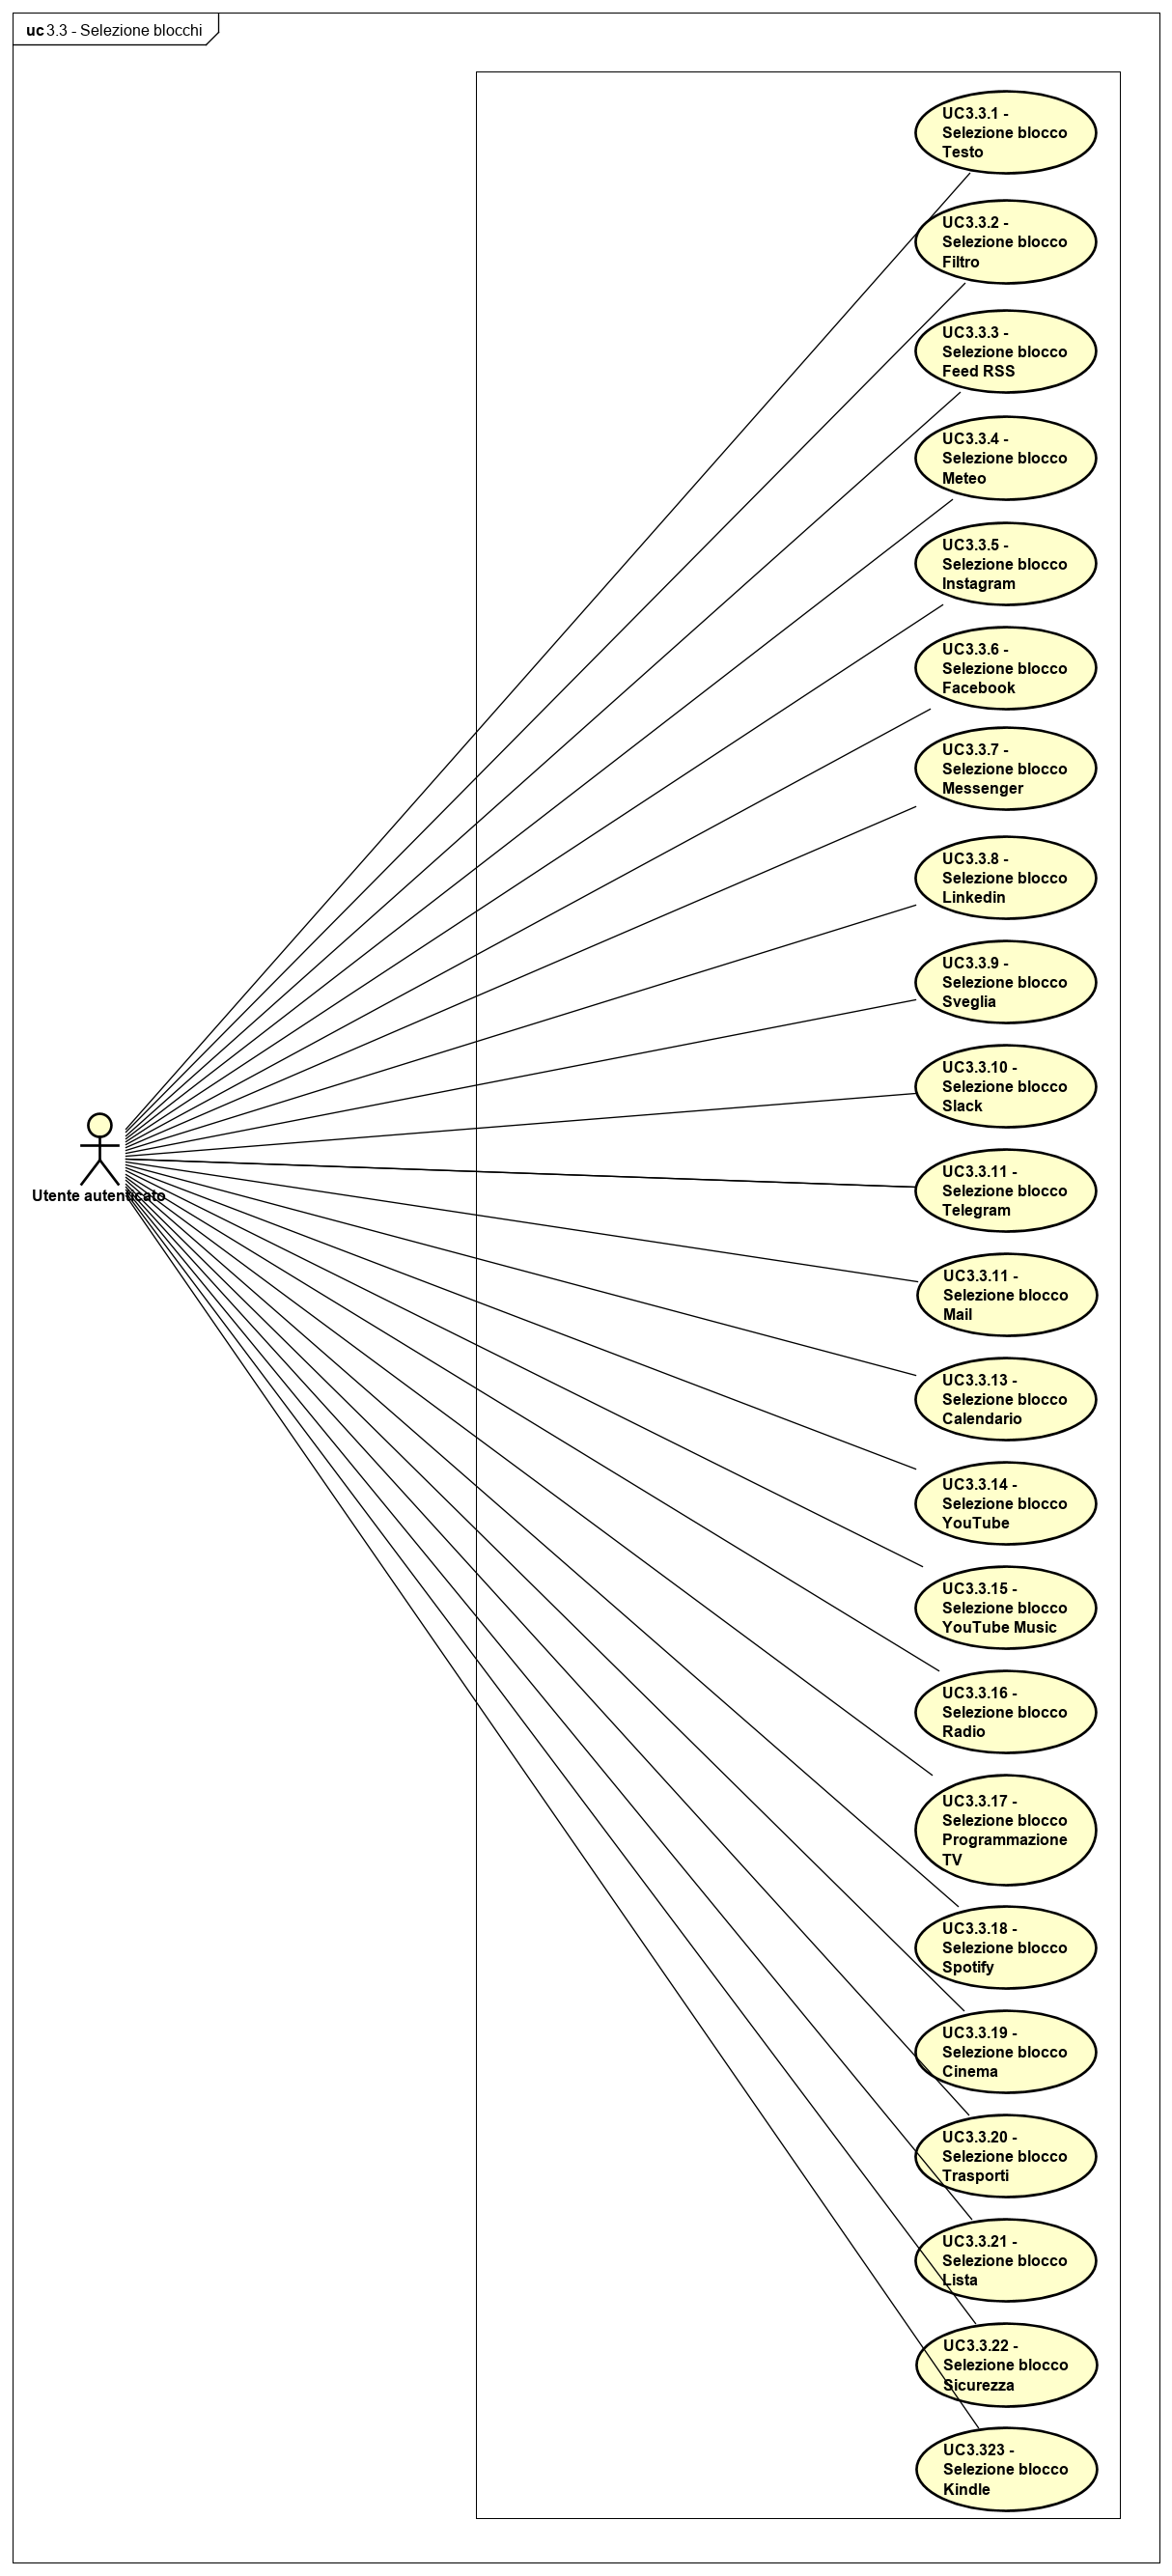
\includegraphics[scale=0.3]{immagini/UC3-3}
\caption{UC3.3 - Selezione blocchi\label{fig:UC3-3}}
\end{figure}

\pagebreak
\subparagraph{UC3.3.1 - Selezione blocco Testo}

\begin{itemize}
\item \textbf{Attori primari}:  utente autenticato;

\item \textbf{Descrizione}: l'attore può inserire un blocco di testo nel workflow. Tale testo verrà letto a voce da Alexa;

\item \textbf{Pre-condizione}: l'attore vuole inserire il \BTesto{} all'interno del workflow;

\item \textbf{Post-condizione}: il \BTesto{} è pronto per essere configurato;

\item \textbf{Scenario principale}:
\begin{enumerate}
\item l'utente può selezionare il \BTesto{}.
\end{enumerate}
\end{itemize}

\subparagraph{UC3.3.2 - Selezione \BFeedRSS{}}

\begin{itemize}
\item \textbf{Attori primari}:  utente autenticato;

\item \textbf{Descrizione}: l'attore può inserire il blocco del feed RSS nel workflow;

\item \textbf{Pre-condizione}: l'attore vuole inserire il \BFeedRSS{} all'interno del workflow;

\item \textbf{Post-condizione}: il \BFeedRSS{} è pronto per essere configurato;

\item \textbf{Scenario principale}:
\begin{enumerate}
\item l'utente può selezionare il \BFeedRSS{}.
\end{enumerate}
\end{itemize}

\subparagraph{UC3.3.3 - Selezione \BFiltro{}}

\begin{itemize}
\item \textbf{Attori primari}:  utente autenticato;

\item \textbf{Descrizione}: l'attore può inserire il \BFiltro{} nel workflow. Tale filtro verrà applicato al risultato del blocco collegato a questo;

\item \textbf{Pre-condizione}: l'attore vuole inserire il \BFiltro{} all'interno del workflow;

\item \textbf{Post-condizione}:  il \BFiltro{} è pronto per essere configurato;

\item \textbf{Scenario principale}:
\begin{enumerate}
\item l'utente può selezionare il \BFiltro{};
\item l'utente collega il \BFiltro{} ad un altro blocco.
\end{enumerate}
\end{itemize}

\subparagraph{UC3.3.4 - Selezione \BMeteo{}}

\begin{itemize}
\item \textbf{Attori primari}: utente autenticato;

\item \textbf{Descrizione}:  l'attore può inserire il \BMeteo{} nel workflow. Tale blocco fornisce il meteo della città in cui ci si trova o di una città inserita dall'utente;

\item \textbf{Pre-condizione}: l'attore vuole inserire il \BMeteo{} all'interno del workflow;

\item \textbf{Post-condizione}: il \BMeteo{} è pronto per essere configurato;

\item \textbf{Scenario principale}:
\begin{enumerate}
\item l'utente può selezionare il \BMeteo{}.

\end{enumerate}
\end{itemize}

\subparagraph{UC3.3.5 - Selezione \BInstagram{}}

\begin{itemize}
\item \textbf{Attori primari}: utente autenticato;

\item \textbf{Descrizione}: l'attore può inserire il \BInstagram{} nel workflow. Tale blocco permette di leggere le notifiche del profilo dell'utente o visualizzare le foto di un certo profilo o di un hashtag selezionato dall'utente;

\item \textbf{Pre-condizione}: l'attore vuole inserire il \BInstagram{} all'interno del workflow;

\item \textbf{Post-condizione}: il \BInstagram{} è pronto per essere configurato;

\item \textbf{Scenario principale}:
\begin{enumerate}
\item l'utente può selezionare il \BInstagram{}.

\end{enumerate}
\end{itemize}

\subparagraph{UC3.3.6 - Selezione \BFacebook{}}

\begin{itemize}
\item \textbf{Attori primari}: utente autenticato;

\item \textbf{Descrizione}: l'attore può inserire il \BFacebook{} nel workflow. Tale blocco permette di leggere le notifiche del profilo Facebook  e gli ultimi post dell'utente;

\item \textbf{Pre-condizione}: l'attore vuole inserire il \BFacebook{} all'interno del workflow;

\item \textbf{Post-condizione}: il \BFacebook{} è pronto per essere configurato;

\item \textbf{Scenario principale}:
\begin{enumerate}
\item l'utente può selezionare il \BFacebook{}.

\end{enumerate}
\end{itemize}

\subparagraph{UC3.3.7 - Selezione \BMessenger{}}

\begin{itemize}
\item \textbf{Attori primari}: utente autenticato;

\item \textbf{Descrizione}:  l'attore può inserire il \BMessenger{} nel workflow. Tale blocco permette di leggere i nuovi messaggi da Facebook Messenger;

\item \textbf{Pre-condizione}: l'attore vuole inserire il \BMessenger{} all'interno del workflow;

\item \textbf{Post-condizione}: il \BMessenger{} è pronto per essere configurato;

\item \textbf{Scenario principale}:
\begin{enumerate}
\item l'utente può selezionare il \BMessenger{}.

\end{enumerate}
\end{itemize}

\subparagraph{UC3.3.8 - Selezione \BLinkedIn{}}

\begin{itemize}
\item \textbf{Attori primari}: utente autenticato;

\item \textbf{Descrizione}: l'attore può inserire il \BLinkedIn{} nel workflow. Tale blocco permette di leggere le nuove notifiche e i nuovi messaggi del profilo LinkedIn dell'utente;

\item \textbf{Pre-condizione}: l'attore vuole inserire il \BLinkedIn{} all'interno del workflow;

\item \textbf{Post-condizione}: il \BLinkedIn{} è pronto per essere configurato;

\item \textbf{Scenario principale}:
\begin{enumerate}
\item l'utente può selezionare il \BLinkedIn{}.

\end{enumerate}
\end{itemize}

\subparagraph{UC3.3.9 - Selezione \BSveglia{}}

\begin{itemize}
\item \textbf{Attori primari}: utente autenticato;

\item \textbf{Descrizione}: l'attore può inserire il \BSveglia{} nel workflow. Tale blocco permette di impostare una sveglia con l'orario e suoneria personalizzata;

\item \textbf{Pre-condizione}: l'attore vuole inserire il \BSveglia{} all'interno del workflow;

\item \textbf{Post-condizione}: il \BSveglia{} è pronto per essere configurato;

\item \textbf{Scenario principale}:
\begin{enumerate}
\item l'utente può selezionare il \BSveglia{}.

\end{enumerate}
\end{itemize}

\subparagraph{UC3.3.10 - Selezione \BSlack{}}

\begin{itemize}
\item \textbf{Attori primari}: utente autenticato;

\item \textbf{Descrizione}: l'attore può inserire il \BSlack{} nel workflow. Tale blocco permette di leggere gli ultimi messaggi da Slack;

\item \textbf{Pre-condizione}: l'attore vuole inserire il \BSlack{} all'interno del workflow;

\item \textbf{Post-condizione}: il \BSlack{} è pronto per essere configurato;

\item \textbf{Scenario principale}:
\begin{enumerate}
\item l'utente può selezionare il \BSlack{}.

\end{enumerate}
\end{itemize}

\subparagraph{UC3.3.11 - Selezione \BTelegram{}}

\begin{itemize}
\item \textbf{Attori primari}: utente autenticato;

\item \textbf{Descrizione}: l'attore può inserire il \BTelegram{} nel workflow. Tale blocco permette di leggere gli ultimi messaggi testuali e riprodurre quelli vocali da Telegram;

\item \textbf{Pre-condizione}: l'attore vuole inserire il \BTelegram{} all'interno del workflow;

\item \textbf{Post-condizione}:  il \BTelegram{} è pronto per essere configurato;

\item \textbf{Scenario principale}:
\begin{enumerate}
\item l'utente può selezionare il \BTelegram{}.

\end{enumerate}
\end{itemize}

\subparagraph{UC3.3.12 - Selezione \BMail{}}

\begin{itemize}
\item \textbf{Attori primari}: utente autenticato;

\item \textbf{Descrizione}: l'attore può inserire il \BMail{} nel workflow. Tale blocco permette di leggere le nuove mail e riferire il numero di mail non lette;

\item \textbf{Pre-condizione}: l'attore vuole inserire il \BMail{} all'interno del workflow;

\item \textbf{Post-condizione}: il \BMail{} è pronto per essere configurato;

\item \textbf{Scenario principale}:
\begin{enumerate}
\item l'utente può inserire il \BMail{} nel workflow.

\end{enumerate}
\end{itemize}

\subparagraph{UC3.3.13 - Selezione \BCalendario{}}

\begin{itemize}
\item \textbf{Attori primari}: utente autenticato;

\item \textbf{Descrizione}: l'attore può inserire il \BCalendario{} nel workflow. Tale blocco permette leggere e inserire eventi nel calendario di Google;

\item \textbf{Pre-condizione}: l'attore vuole inserire il \BCalendario{} all'interno del workflow;

\item \textbf{Post-condizione}: il \BCalendario{} è pronto per essere configurato;

\item \textbf{Scenario principale}:
\begin{enumerate}
\item l'utente può selezionare il \BCalendario{}.

\end{enumerate}
\end{itemize}

\subparagraph{UC3.3.14 - Selezione \BYouTube{}}

\begin{itemize}
\item \textbf{Attori primari}: utente autenticato;

\item \textbf{Descrizione}: l'attore può inserire il \BYouTube{} nel workflow. Tale blocco permette la riproduzione degli ultimi video caricati da un canale YouTube inserito dall'utente;

\item \textbf{Pre-condizione}: l'attore vuole inserire il \BYouTube{} all'interno del workflow;

\item \textbf{Post-condizione}: il \BYouTube{} è pronto per essere configurato;

\item \textbf{Scenario principale}:
\begin{enumerate}
\item  l'utente può inserire il \BYouTube{} nel workflow.

\end{enumerate}
\end{itemize}

\subparagraph{UC3.3.15 - Selezione \BYouTubeMusic{}}

\begin{itemize}
\item \textbf{Attori primari}: utente autenticato;

\item \textbf{Descrizione}: l'attore può inserire il \BYouTubeMusic{} nel workflow. Tale blocco permette di riprodurre musica tramite YouTube Music;

\item \textbf{Pre-condizione}: l'attore vuole inserire il \BYouTubeMusic{} all'interno del workflow;

\item \textbf{Post-condizione}: il \BYouTubeMusic{} è pronto per essere configurato;

\item \textbf{Scenario principale}:
\begin{enumerate}
\item  l'utente può selezionare il \BYouTubeMusic{}.

\end{enumerate}
\end{itemize}

\subparagraph{UC3.3.16 - Selezione \BRadio{}}

\begin{itemize}
\item \textbf{Attori primari}: utente autenticato;

\item \textbf{Descrizione}: l'attore può inserire il \BRadio{} nel workflow. Tale blocco permette di riprodurre una radio a scelta tra quelle proposte;

\item \textbf{Pre-condizione}: l'attore vuole inserire il \BRadio{} all'interno del workflow;

\item \textbf{Post-condizione}: il \BRadio{} è pronto per essere configurato;

\item \textbf{Scenario principale}:
\begin{enumerate}
\item  l'utente può selezionare il \BRadio{}.

\end{enumerate}
\end{itemize}

\subparagraph{UC3.3.17 - Selezione \BTV{}}

\begin{itemize}
\item \textbf{Attori primari}: utente autenticato;

\item \textbf{Descrizione}: l'attore può inserire il \BTV{} nel workflow. Tale blocco permette di leggere la programmazione di un canale TV;

\item \textbf{Pre-condizione}: l'attore vuole inserire il \BTV{} all'interno del workflow;

\item \textbf{Post-condizione}: il \BTV{} è pronto per essere configurato;

\item \textbf{Scenario principale}:
\begin{enumerate}
\item  l'utente può selezionare il \BTV{}.

\end{enumerate}
\end{itemize}

\subparagraph{UC3.3.18 - Selezione \BSpotify{}}

\begin{itemize}
\item \textbf{Attori primari}: utente autenticato;

\item \textbf{Descrizione}: l'attore può inserire il \BSpotify{} nel workflow. Tale blocco permette di riprodurre musica tramite Spotify;

\item \textbf{Pre-condizione}: l'attore vuole inserire il \BSpotify{} all'interno del workflow;

\item \textbf{Post-condizione}: il \BSpotify{} è pronto per essere configurato;

\item \textbf{Scenario principale}:
\begin{enumerate}
\item  l'utente può selezionare il \BSpotify{}.

\end{enumerate}
\end{itemize}

\subparagraph{UC3.3.19 - Selezione \BCinema{}}

\begin{itemize}
\item \textbf{Attori primari}: utente autenticato;

\item \textbf{Descrizione}: l'attore può inserire il \BCinema{} nel workflow. Tale blocco permette di visualizzare la programmazione di un cinema scelto dall'utente;

\item \textbf{Pre-condizione}: l'attore vuole inserire il \BCinema{} all'interno del workflow;

\item \textbf{Post-condizione}: il \BCinema{} è pronto per essere configurato;

\item \textbf{Scenario principale}:
\begin{enumerate}
\item  l'utente può selezionare il \BCinema{}.

\end{enumerate}
\end{itemize}

\subparagraph{UC3.3.20 - Selezione \BTrasporti{}}

\begin{itemize}
\item \textbf{Attori primari}: utente autenticato;

\item \textbf{Descrizione}: l'attore può inserire il \BTrasporti{} nel workflow. Tale blocco permette di visualizzare le varie informazioni riguardo ai mezzi di trasporto tra quelli selezionati;

\item \textbf{Pre-condizione}: l'attore vuole inserire il \BCinema{} all'interno del workflow;

\item \textbf{Post-condizione}: il \BTrasporti{} è pronto per essere configurato;

\item \textbf{Scenario principale}:
\begin{enumerate}
\item  l'utente può selezionare il \BTrasporti{}.

\end{enumerate}
\end{itemize}

\subparagraph{UC3.3.21 - Selezione \BLista{}}

\begin{itemize}
\item \textbf{Attori primari}: utente autenticato;

\item \textbf{Descrizione}:  l'attore può inserire il \BLista{} nel workflow. Tale blocco permette di aggiungere elementi ad una lista;

\item \textbf{Pre-condizione}: l'attore vuole inserire il \BLista{} all'interno del workflow;

\item \textbf{Post-condizione}: il \BLista{} è pronto per essere configurato;

\item \textbf{Scenario principale}:
\begin{enumerate}
\item  l'utente può selezionare il \BLista{}.

\end{enumerate}
\end{itemize}

\subparagraph{UC3.3.22 - Selezione \BSicurezza{}}

\begin{itemize}
\item \textbf{Attori primari}: utente autenticato;

\item \textbf{Descrizione}:  l'attore può inserire il \BSicurezza{} nel workflow. Tale blocco permette impostare un PIN di sicurezza per il workflow;

\item \textbf{Pre-condizione}: l'attore vuole inserire il \BSicurezza{} all'interno del workflow;

\item \textbf{Post-condizione}: il \BSicurezza{} è pronto per essere configurato;

\item \textbf{Scenario principale}:
\begin{enumerate}
\item  l'utente può selezionare il \BSicurezza{}.

\end{enumerate}
\end{itemize}

\subparagraph{UC3.3.23 - Selezione \BKindle{}}

\begin{itemize}
\item \textbf{Attori primari}: utente autenticato;

\item \textbf{Descrizione}:  l'attore può inserire il \BKindle{} nel workflow. Tale blocco permette ad Alexa di poter leggere file testuale in formato PDF e EPUB;

\item \textbf{Pre-condizione}: l'attore vuole inserire il \BKindle{} all'interno del workflow;

\item \textbf{Post-condizione}: il \BKindle{} è pronto per essere configurato;

\item \textbf{Scenario principale}:
\begin{enumerate}
\item  l'utente può selezionare il \BKindle{}.

\end{enumerate}
\end{itemize}

\pagebreak

\paragraph{UC3.4 - Configurazione blocchi}
\begin{figure}[htbp]
\centering
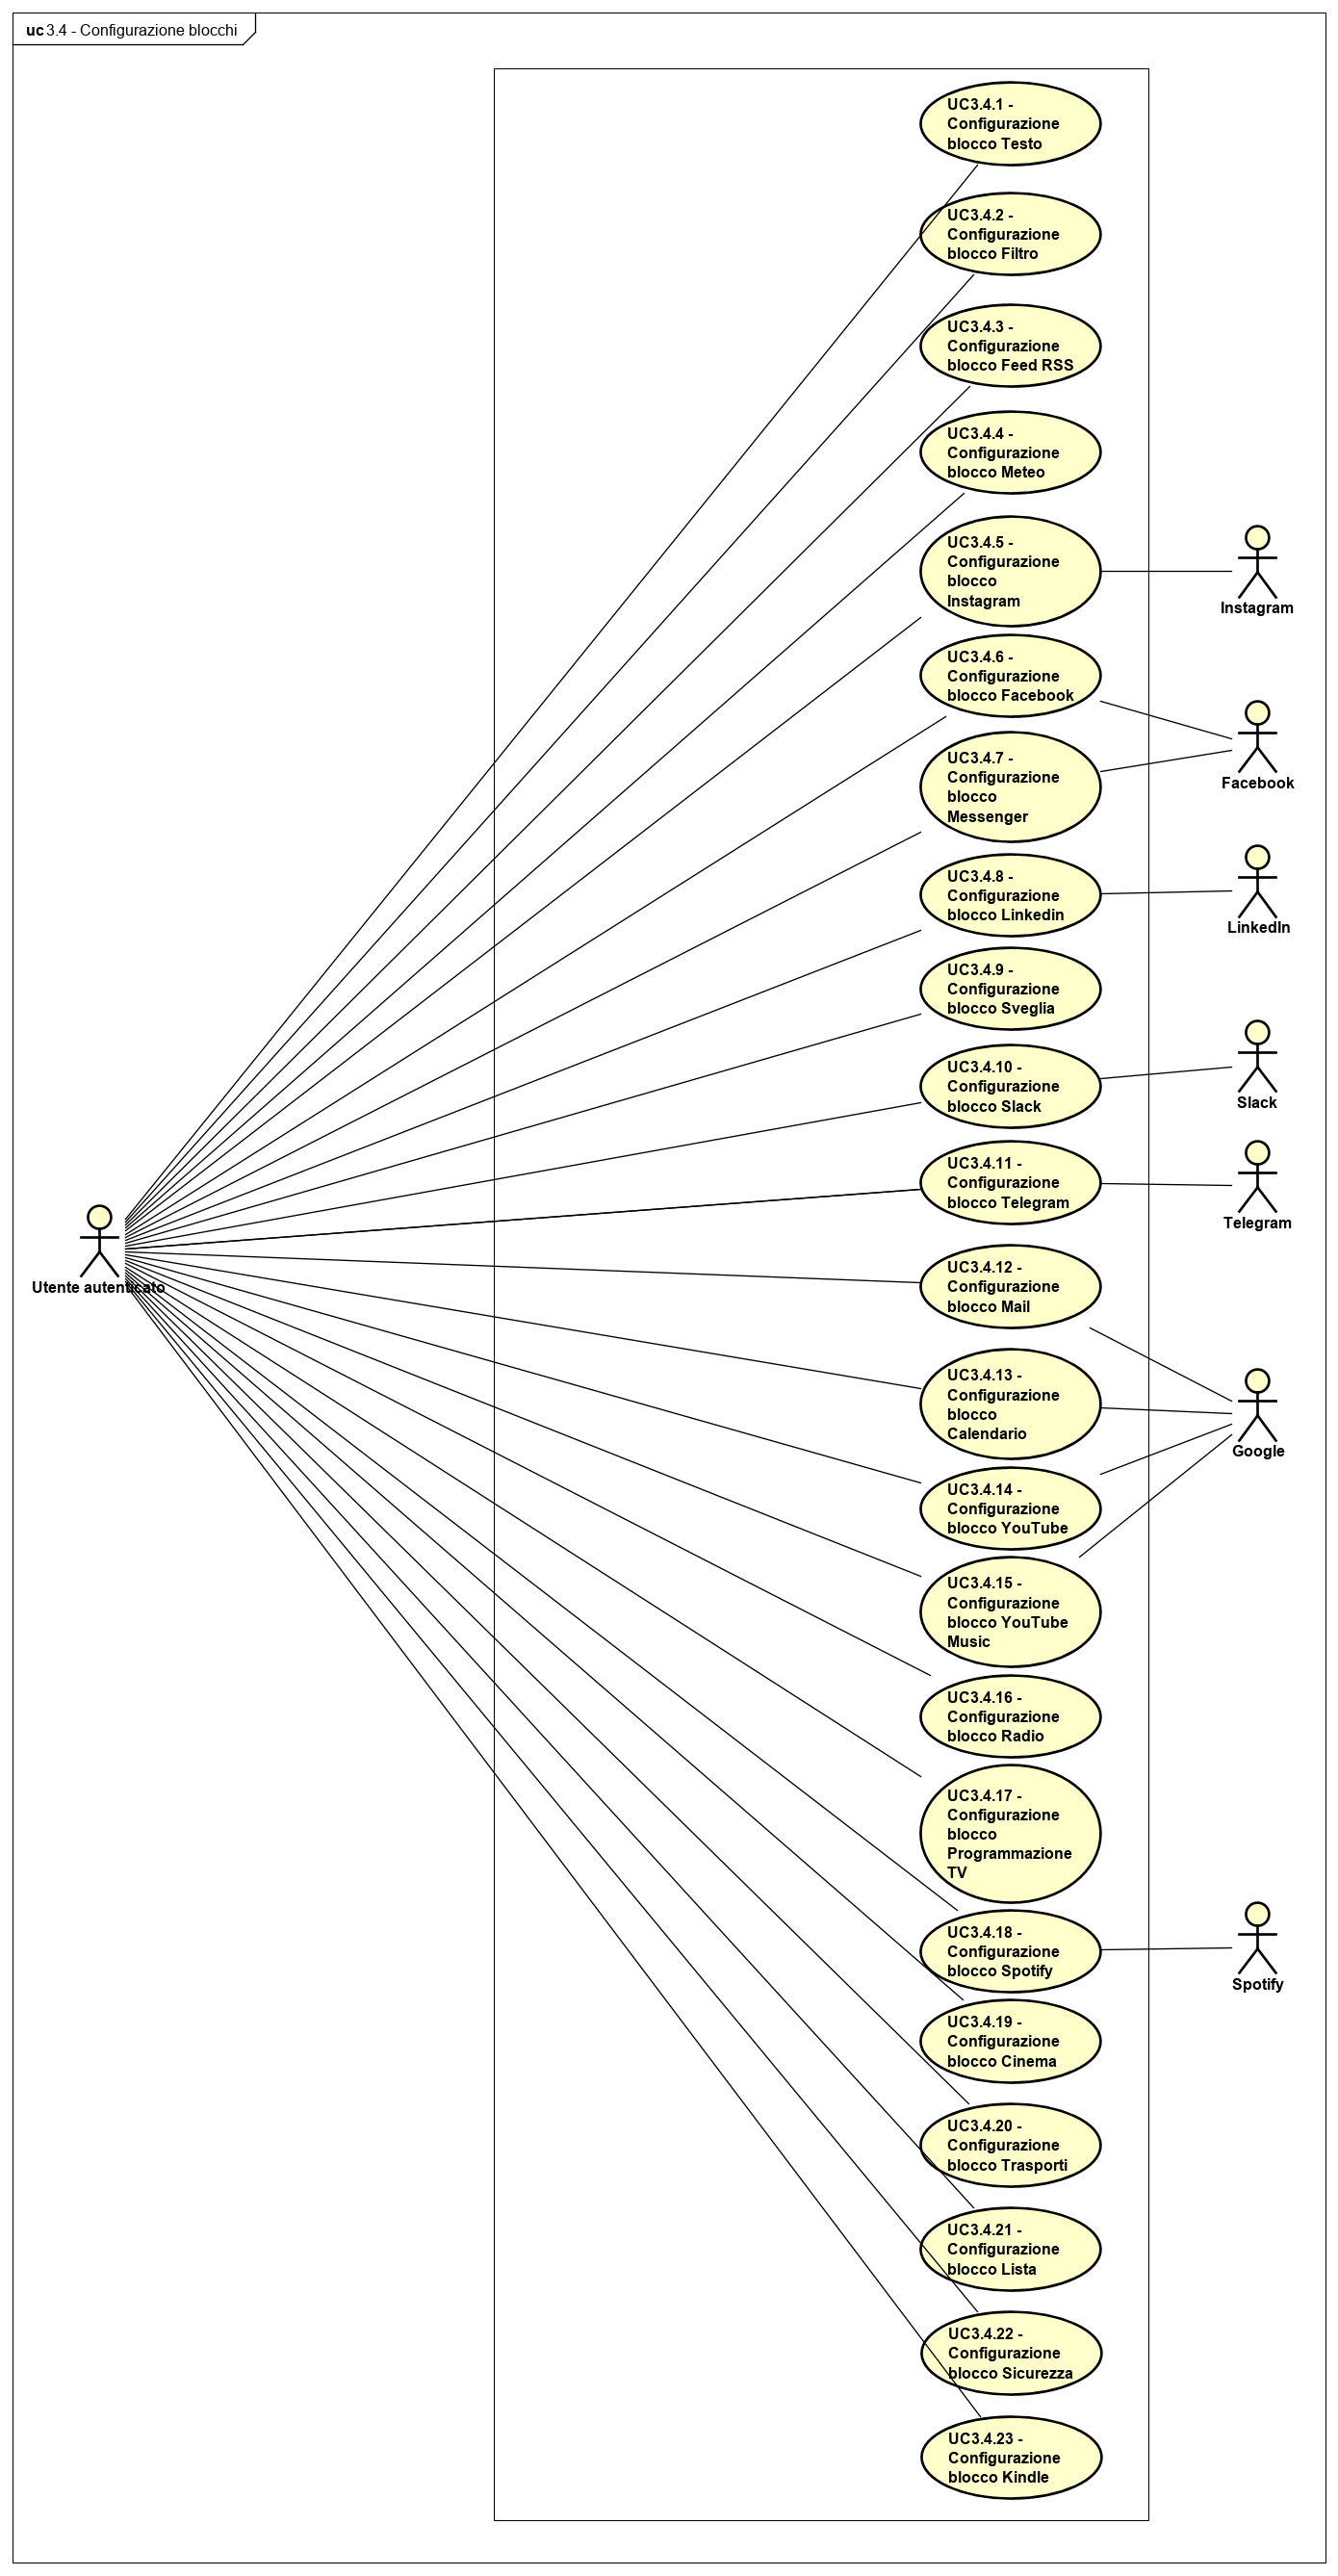
\includegraphics[scale=0.30]{immagini/UC3-4}
\caption{UC3.4 - Configurazione blocchi \label{fig:UC3-4}}
\end{figure}

\begin{itemize}
\item \textbf{Attori primari}: utente autenticato;

\item \textbf{Attori secondari}: Instagram, Facebook, LinkedIn, Slack, Telegram, Google, Spotify;

\item \textbf{Descrizione}: l'attore può configurare i blocchi inseriti nel workflow;

\item \textbf{Pre-condizione}: Sono presenti blocchi da configurare;

\item \textbf{Post-condizione}:  i blocchi sono stati configurati;

\item \textbf{Scenario principale}:
\begin{enumerate}
\item l'utente può configurare il blocco Testo (UC3.4.1);
\item l'utente può configurare il \BFeedRSS{} (UC3.4.2);
\item l'utente può configurare il \BFiltro{} (UC3.4.3);
\item l'utente può configurare il \BMeteo{} (UC3.4.4);
\item l'utente può configurare il \BInstagram{} (UC3.4.5);
\item l'utente può configurare il \BFacebook{} (UC3.4.6);
\item l'utente può configurare il \BMessenger{} (UC3.4.7);
\item l'utente può configurare il \BLinkedIn{} (UC3.4.8);
\item l'utente può configurare il \BSveglia{} (UC3.4.9);
\item l'utente può configurare il \BSlack{} (UC3.4.10);
\item l'utente può configurare il \BTelegram{} (UC3.4.11);
\item l'utente può configurare il \BMail{} (UC3.4.12);
\item l'utente può configurare il \BCalendario{} (UC3.4.13);
\item l'utente può configurare il \BYouTube{} (UC3.4.14);
\item l'utente può configurare il \BYouTubeMusic{} (UC3.4.15);
\item l'utente può configurare il \BRadio{} (UC3.4.16);
\item l'utente può configurare il \BTV{} (UC3.4.17);
\item l'utente può configurare il \BSpotify{} (UC3.4.18);
\item l'utente può configurare il \BCinema{} (UC3.4.19);
\item l'utente può configurare il \BTrasporti{} (UC3.4.20);
\item l'utente può configurare il \BLista{} (UC3.4.21);
\item l'utente può configurare il \BSicurezza{} (UC3.4.22);
\item l'utente può configurare il \BKindle{} (UC3.4.23).

\end{enumerate}
\end{itemize}

\subparagraph{UC3.4.1 - Configurazione blocco Testo}

\begin{itemize}
\item \textbf{Attori primari}: utente autenticato;

\item \textbf{Descrizione}: l'attore può scrivere un testo che verrà letto a voce da Alexa;

\item \textbf{Pre-condizione}: l'attore vuole configurare il blocco Testo;

\item \textbf{Post-condizione}: il blocco è stato configurato correttamente;

\item \textbf{Scenario principale}:
\begin{enumerate}
\item  l'utente può configurare il blocco Testo.

\end{enumerate}
\end{itemize}

\subparagraph{UC3.4.2 - Configurazione \BFeedRSS{}}

\begin{itemize}
\item \textbf{Attori primari}: utente autenticato;

\item \textbf{Descrizione}: l'attore può inserire l'URL di un Feed RSS;

\item \textbf{Pre-condizione}: l'attore vuole configurare il \BFeedRSS{};

\item \textbf{Post-condizione}: il blocco è stato configurato correttamente;

\item \textbf{Scenario principale}:
\begin{enumerate}
\item  l'utente può configurare il \BFeedRSS{}.

\end{enumerate}
\end{itemize}

\subparagraph{UC3.4.3 - Configurazione \BFiltro{}}

\begin{itemize}
\item \textbf{Attori primari}: utente autenticato;

\item \textbf{Descrizione}: l'attore può configurare un filtro collegabile ad un blocco. Vengono visualizzati i filtri specifici di quel blocco;

\item \textbf{Pre-condizione}: l'attore vuole configurare il \BFiltro{};

\item \textbf{Post-condizione}:  il blocco è stato configurato correttamente;

\item \textbf{Scenario principale}:
\begin{enumerate}
\item  l'utente può configurare il \BFiltro{}.

\end{enumerate}
\end{itemize}

\subparagraph{UC3.4.4 - Configurazione \BMeteo{}}

\begin{itemize}
\item \textbf{Attori primari}: utente autenticato;

\item \textbf{Descrizione}: l'attore può configurare il \BMeteo{} tramite inserimento testuale di una località o tramite geolocalizzazione;

\item \textbf{Pre-condizione}: l'attore vuole configurare il \BMeteo{};

\item \textbf{Post-condizione}:  il blocco è stato configurato correttamente;

\item \textbf{Scenario principale}:
\begin{enumerate}
\item  l'utente può configurare il \BMeteo{}.

\end{enumerate}
\end{itemize}

\subparagraph{UC3.4.5 - Configurazione \BInstagram{}}

\begin{itemize}
\item \textbf{Attori primari}: utente autenticato;

\item \textbf{Attori secondari}: Instagram;

\item \textbf{Descrizione}: l'attore può inserire le credenziali dell'account Instagram e il profilo o l'hashtag di cui si vuole vedere le foto;

\item \textbf{Pre-condizione}: l'attore vuole configurare il \BInstagram{};

\item \textbf{Post-condizione}:  il blocco è stato configurato correttamente;

\item \textbf{Scenario principale}:
\begin{enumerate}
\item  l'utente può configurare il \BInstagram{}.

\end{enumerate}
\end{itemize}

\subparagraph{UC3.4.6 - Configurazione \BFacebook{}}

\begin{itemize}
\item \textbf{Attori primari}: utente autenticato;

\item \textbf{Attori secondari}: Facebook;

\item \textbf{Descrizione}: l'attore inserire le credenziali dell'account Facebook;

\item \textbf{Pre-condizione}: l'attore vuole configurare il \BFacebook{};

\item \textbf{Post-condizione}:  il blocco è stato configurato correttamente;

\item \textbf{Scenario principale}:
\begin{enumerate}
\item  l'utente può configurare il \BFacebook{}.

\end{enumerate}
\end{itemize}

\subparagraph{UC3.4.7 - Configurazione \BMessenger{}}

\begin{itemize}
\item \textbf{Attori primari}: utente autenticato;

\item \textbf{Attori secondari}: Facebook;

\item \textbf{Descrizione}: l'attore può inserire le credenziali dell'account Facebook;

\item \textbf{Pre-condizione}: l'attore vuole configurare il \BMessenger{};

\item \textbf{Post-condizione}:  il blocco è stato configurato correttamente;

\item \textbf{Scenario principale}:
\begin{enumerate}
\item  l'utente può configurare il \BMessenger{}.

\end{enumerate}
\end{itemize}

\subparagraph{UC3.4.8 - Configurazione \BLinkedIn{}}

\begin{itemize}
\item \textbf{Attori primari}: utente autenticato;

\item \textbf{Attori secondari}: LinkedIn;

\item \textbf{Descrizione}: l'attore può inserire le credenziali dell'account LinkedIn;

\item \textbf{Pre-condizione}: l'attore vuole configurare il \BLinkedIn{};

\item \textbf{Post-condizione}:  il blocco è stato configurato correttamente;

\item \textbf{Scenario principale}:
\begin{enumerate}
\item  l'utente può configurare il \BLinkedIn{}.

\end{enumerate}
\end{itemize}

\subparagraph{UC3.4.9 - Configurazione \BSveglia{}}

\begin{itemize}
\item \textbf{Attori primari}: utente autenticato;

\item \textbf{Descrizione}: l'attore può inserire un orario e selezionare una suoneria personalizzata;

\item \textbf{Pre-condizione}: l'attore vuole configurare il \BSveglia{};

\item \textbf{Post-condizione}:  il blocco è stato configurato correttamente;

\item \textbf{Scenario principale}:
\begin{enumerate}
\item  l'utente può configurare il \BSveglia{}.

\end{enumerate}
\end{itemize}

\subparagraph{UC3.4.10 - Configurazione \BSlack{}}

\begin{itemize}
\item \textbf{Attori primari}: utente autenticato;

\item \textbf{Attori secondari}: Slack;

\item \textbf{Descrizione}: l'attore può inserire le credenziali dell'account Slack e l'URL del gruppo di lavoro;

\item \textbf{Pre-condizione}: l'attore vuole configurare il \BSlack{};

\item \textbf{Post-condizione}:  il blocco è stato configurato correttamente;

\item \textbf{Scenario principale}:
\begin{enumerate}
\item  l'utente può configurare il \BSlack{}.

\end{enumerate}
\end{itemize}

\subparagraph{UC3.4.11 - Configurazione \BTelegram{}}

\begin{itemize}
\item \textbf{Attori primari}: utente autenticato;

\item \textbf{Attori secondari}: Telegram;

\item \textbf{Descrizione}: l'attore può inserire il numero di telefono cellulare collegato all'account Telegram;

\item \textbf{Pre-condizione}: l'attore vuole configurare il \BTelegram{};

\item \textbf{Post-condizione}:  il blocco è stato configurato correttamente;

\item \textbf{Scenario principale}:
\begin{enumerate}
\item  l'utente può configurare il \BTelegram{}.

\end{enumerate}
\end{itemize}

\subparagraph{UC3.4.12 - Configurazione \BMail{}}

\begin{itemize}
\item \textbf{Attori primari}: utente autenticato;

\item \textbf{Attori secondari}: Google;

\item \textbf{Descrizione}: l'attore può inserire le credenziali dell'account Google;

\item \textbf{Pre-condizione}: l'attore vuole configurare il \BMail{};

\item \textbf{Post-condizione}:  il blocco è stato configurato correttamente;

\item \textbf{Scenario principale}:
\begin{enumerate}
\item  l'utente può configurare il \BMail{}.

\end{enumerate}
\end{itemize}

\subparagraph{UC3.4.13 - Configurazione \BCalendario{}}

\begin{itemize}
\item \textbf{Attori primari}: utente autenticato;

\item \textbf{Attori secondari}: Google;

\item \textbf{Descrizione}: l'attore può inserire le credenziali dell'account Google e inserire l'ora, data e descrizione dell'evento da inserire;

\item \textbf{Pre-condizione}: l'attore vuole configurare il \BCalendario{};

\item \textbf{Post-condizione}:  il blocco è stato configurato correttamente;

\item \textbf{Scenario principale}:
\begin{enumerate}
\item  l'utente può configurare il \BCalendario{}.

\end{enumerate}
\end{itemize}

\subparagraph{UC3.4.14 - Configurazione \BYouTube{}}

\begin{itemize}
\item \textbf{Attori primari}: utente autenticato;

\item \textbf{Attori secondari}: Google;

\item \textbf{Descrizione}: l'attore può inserire le credenziali dell'account Google e l'URL di un canale YouTube;

\item \textbf{Pre-condizione}: l'attore vuole configurare il \BYouTube{};

\item \textbf{Post-condizione}:  il blocco è stato configurato correttamente;

\item \textbf{Scenario principale}:
\begin{enumerate}
\item  l'utente può configurare il \BYouTube{}.

\end{enumerate}
\end{itemize}

\subparagraph{UC3.4.15 - Configurazione \BYouTubeMusic{}}

\begin{itemize}
\item \textbf{Attori primari}: utente autenticato;

\item \textbf{Attori secondari}: Google;

\item \textbf{Descrizione}: l'attore può inserire le credenziali dell'account Google e l'URL di un canale YouTube Music, di una playlist o di una canzone;

\item \textbf{Pre-condizione}: l'attore vuole configurare il \BYouTubeMusic{};

\item \textbf{Post-condizione}:  il blocco è stato configurato correttamente;

\item \textbf{Scenario principale}:
\begin{enumerate}
\item  l'utente può configurare il \BYouTubeMusic{}.

\end{enumerate}
\end{itemize}

\subparagraph{UC3.4.16 - Configurazione \BRadio{}}

\begin{itemize}
\item \textbf{Attori primari}: utente autenticato;

\item \textbf{Descrizione}: l'attore può selezionare il canale radio preferito;

\item \textbf{Pre-condizione}: l'attore vuole configurare il \BRadio{};

\item \textbf{Post-condizione}:  il blocco è stato configurato correttamente;

\item \textbf{Scenario principale}:
\begin{enumerate}
\item  l'utente può configurare il \BRadio{}.

\end{enumerate}
\end{itemize}

\subparagraph{UC3.4.17 - Configurazione \BTV{}}

\begin{itemize}
\item \textbf{Attori primari}: utente autenticato;

\item \textbf{Descrizione}: l'attore può selezionare il canale TV preferito;

\item \textbf{Pre-condizione}: l'attore vuole configurare il \BTV{};

\item \textbf{Post-condizione}:  il blocco è stato configurato correttamente;

\item \textbf{Scenario principale}:
\begin{enumerate}
\item  l'utente può configurare il \BTV{}.

\end{enumerate}
\end{itemize}

\subparagraph{UC3.4.18 - Configurazione \BSpotify{}}

\begin{itemize}
\item \textbf{Attori primari}: utente autenticato;

\item \textbf{Attori secondari}: Spotify;

\item \textbf{Descrizione}: l'attore può inserire le credenziali dell'account Spotify e la playlist o la canzone desiderata;

\item \textbf{Pre-condizione}: l'attore vuole configurare il \BSpotify{};

\item \textbf{Post-condizione}:  il blocco è stato configurato correttamente;

\item \textbf{Scenario principale}:
\begin{enumerate}
\item  l'utente può configurare il \BSpotify{}.

\end{enumerate}
\end{itemize}

\subparagraph{UC3.4.19 - Configurazione \BCinema{}}

\begin{itemize}
\item \textbf{Attori primari}: utente autenticato;

\item \textbf{Descrizione}: l'attore può configurare il \BCinema{} tramite inserimento testuale di una località o tramite geolocalizzazione;

\item \textbf{Pre-condizione}: l'attore vuole configurare il \BCinema{};

\item \textbf{Post-condizione}:  il blocco è stato configurato correttamente;

\item \textbf{Scenario principale}:
\begin{enumerate}
\item  l'utente può configurare il \BCinema{}.

\end{enumerate}
\end{itemize}

\subparagraph{UC3.4.20 - Configurazione \BTrasporti{}}

\begin{itemize}
\item \textbf{Attori primari}: utente autenticato;

\item \textbf{Descrizione}: l'attore può configurare il \BTrasporti{} tramite inserimento testuale della città di partenza e arrivo;

\item \textbf{Pre-condizione}: l'attore vuole configurare il \BTrasporti{};

\item \textbf{Post-condizione}:  il blocco è stato configurato correttamente;

\item \textbf{Scenario principale}:
\begin{enumerate}
\item  l'utente può configurare il \BTrasporti{}.

\end{enumerate}
\end{itemize}

\subparagraph{UC3.4.21 - Configurazione \BLista{}}

\begin{itemize}
\item \textbf{Attori primari}: utente autenticato;

\item \textbf{Descrizione}: l'attore può inserire e modificare un elemento nella lista;

\item \textbf{Pre-condizione}: l'attore vuole configurare il \BLista{};

\item \textbf{Post-condizione}:  il blocco è stato configurato correttamente;

\item \textbf{Scenario principale}:
\begin{enumerate}
\item  l'utente può configurare il \BLista{}.

\end{enumerate}
\end{itemize}

\subparagraph{UC3.4.22 - Configurazione \BSicurezza{}}

\begin{itemize}
\item \textbf{Attori primari}: utente autenticato;

\item \textbf{Descrizione}: l'attore può inserire un PIN al workflow;

\item \textbf{Pre-condizione}: l'attore vuole configurare il \BSicurezza{};

\item \textbf{Post-condizione}:  il blocco è stato configurato correttamente;

\item \textbf{Scenario principale}:
\begin{enumerate}
\item  l'utente può configurare il \BSicurezza{}.

\end{enumerate}
\end{itemize}

\subparagraph{UC3.4.23 - Configurazione \BKindle{}}

\begin{itemize}
\item \textbf{Attori primari}: utente autenticato;

\item \textbf{Descrizione}: l'attore può inserire un file PDF o EPUB oppure un link ad un file PDF o EPUB;

\item \textbf{Pre-condizione}: l'attore vuole configurare il \BKindle{};

\item \textbf{Post-condizione}:  il blocco è stato configurato correttamente;

\item \textbf{Scenario principale}:
\begin{enumerate}
\item  l'utente può configurare il \BKindle{}.

\end{enumerate}
\end{itemize}

\subsubsection{UC3.5 - Conferma configurazione workflow}

\begin{itemize}
\item \textbf{Attori primari}: utente autenticato;

\item \textbf{Descrizione}: l'attore può confermare la creazione del workflow;

\item \textbf{Pre-condizione}: l'attore ha finito di configurare il proprio workflow;

\item \textbf{Post-condizione}: i dati vengono salvati dal sistema;

\item \textbf{Scenario principale}:
\begin{enumerate}
\item l'utente clicca il pulsante di conferma.
\end{enumerate}
\item \textbf{Estensione}: viene visualizzato il messaggio di errore configurazione (UC3.6).
\end{itemize}

\subsubsection{UC3.6 - Errore configurazione}

\begin{itemize}
\item \textbf{Attori primari}: utente autenticato;

\item \textbf{Descrizione}: viene visualizzato un errore a video se il nome del workflow è già stato impostato in un altro workflow dell'utente oppure se il nome è vuoto;

\item \textbf{Pre-condizione}: l'attore ha confermato e il nome è errato;

\item \textbf{Post-condizione}: viene visualizzato l'errore a video;

\item \textbf{Scenario principale}:
\begin{enumerate}
\item viene visualizzato l'errore a video di errata configurazione.
\end{enumerate}
\end{itemize}

\subsection{UC4 - Modifica workflow}

\begin{figure}[H]
    \centering
    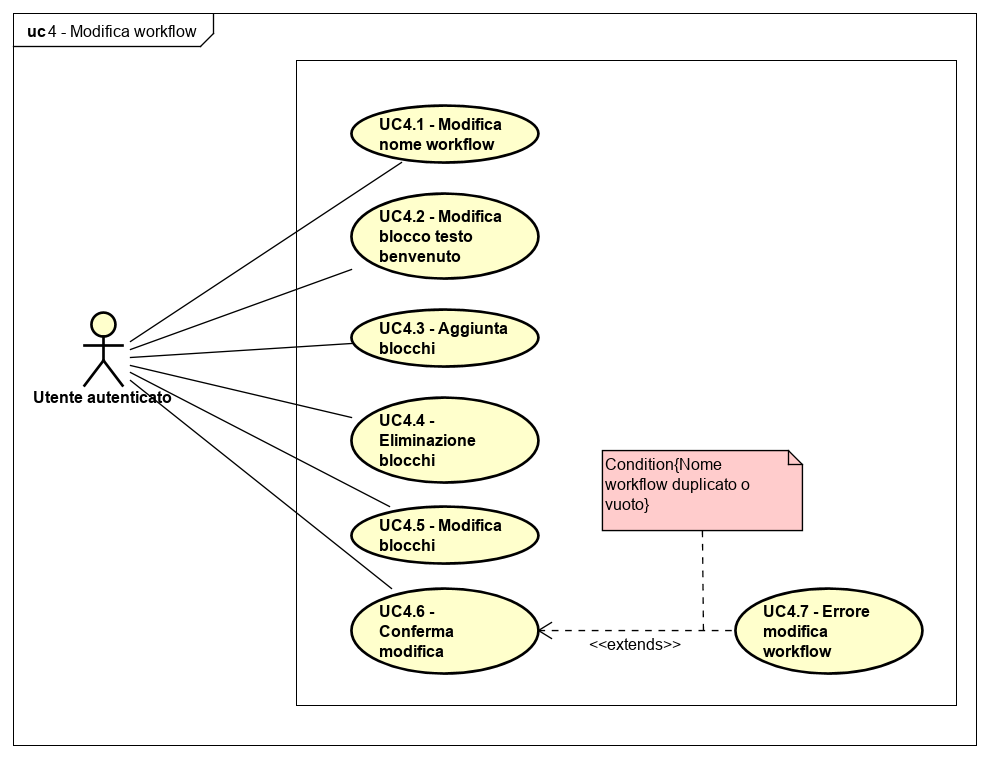
\includegraphics[scale=0.45]{immagini/UC4.png}
    \caption{UC4 - Modifica workflow \label{fig:uc4}}
\end{figure}

\begin{itemize}
\item \textbf{Attori primari}: utente autenticato;

\item \textbf{Descrizione}: l'attore può modificare i workflow precedentemente creati;

\item \textbf{Pre-condizione}: l'attore vuole modificare un workflow;

\item \textbf{Post-condizione}: il workflow è stato modificato e i dati sono stati salvati dal sistema

\item \textbf{Scenario principale}:
\begin{enumerate}
\item l'utente può modificare il nome del workflow (UC4.1);
\item l'utente può modificare il blocco di testo di benvenuto (UC4.2);
\item l'utente può aggiungere nuovi blocchi al workflow (UC4.3);
\item l'utente può eliminare blocchi esistenti dal workflow (UC4.4);
\item l'utente può modificare i blocchi del workflow (UC4.5);
\item l'utente può confermare le modifiche fatte al workflow (UC4.6).
\end{enumerate}
\item \textbf{Estensione}: viene visualizzato un errore a video se i dati sono sbagliati (UC4.7).
\end{itemize}

\subsubsection{UC4.1 - Modifica nome workflow}

\begin{itemize}
\item \textbf{Attori primari}: utente autenticato;

\item \textbf{Descrizione}: l'attore può modificare il nome del workflow;

\item \textbf{Pre-condizione}: l'attore vuole modificare il nome del workflow;

\item \textbf{Post-condizione}: il nome del workflow è stato modificato;

\item \textbf{Scenario principale}:
\begin{enumerate}
\item l'utente può modificare il nome del workflow.
\end{enumerate}
\end{itemize}

\subsubsection{UC4.2 - Modifica blocco testo benvenuto}

\begin{itemize}
\item \textbf{Attori primari}: utente autenticato;

\item \textbf{Descrizione}: l'attore può modificare il testo di benvenuto al workflow;

\item \textbf{Pre-condizione}: l'attore vuole modificare il testo di benvenuto;

\item \textbf{Post-condizione}: il testo del blocco di benvenuto è stato modificato;

\item \textbf{Scenario principale}:
\begin{enumerate}
\item l'utente può modificare il testo di benvenuto.
\end{enumerate}
\end{itemize}

\subsubsection{UC4.3 - Aggiunta blocchi}

\begin{itemize}
\item \textbf{Attori primari}: utente autenticato;

\item \textbf{Descrizione}: l'attore può aggiungere blocchi al workflow. la modalità di aggiunta blocchi è identica a quella descritta nell'UC3.3;

\item \textbf{Pre-condizione}: l'attore vuole aggiungere blocchi al workflow;

\item \textbf{Post-condizione}: i blocchi sono stati aggiunti;

\item \textbf{Scenario principale}:
\begin{enumerate}
\item l'utente può aggiungere blocchi al workflow.
\end{enumerate}
\end{itemize}

\subsubsection{UC4.4 - Eliminazione blocchi}

\begin{itemize}
\item \textbf{Attori primari}: utente autenticato;

\item \textbf{Descrizione}: l'attore può eliminare dei blocchi dal workflow;

\item \textbf{Pre-condizione}: l'attore vuole eliminare dei blocchi dal workflow;

\item \textbf{Post-condizione}: il blocco è stato eliminato dal workflow;

\item \textbf{Scenario principale}:
\begin{enumerate}
\item l'utente può eliminare blocchi dal workflow.
\end{enumerate}
\end{itemize}

\subsubsection{UC4.5 - Modifica blocchi}

\begin{itemize}
\item \textbf{Attori primari}: utente autenticato;

\item \textbf{Descrizione}: l'attore può modificare dei blocchi del workflow. la modalità di modifica dei blocchi è identica a quella descritta nell'UC3.4;

\item \textbf{Pre-condizione}: l'attore vuole modificare dei blocchi nel workflow;

\item \textbf{Post-condizione}: il blocco è stato modificato;

\item \textbf{Scenario principale}:
\begin{enumerate}
\item l'utente può modificare i blocchi del workflow;
\end{enumerate}
\end{itemize}

\subsubsection{UC4.6 - Conferma modifica}

\begin{itemize}
\item \textbf{Attori primari}: utente autenticato;

\item \textbf{Descrizione}: l'attore può confermare le modifiche effettuate;

\item \textbf{Pre-condizione}: l'attore vuole confermare le modifiche effettuate;

\item \textbf{Post-condizione}: le modifiche sono state effettuate e i dati vengono salvati nel sistema;

\item \textbf{Scenario principale}:
\begin{enumerate}
\item l'utente può confermare le modifiche.
\end{enumerate}
\item \textbf{Estensione}: viene visualizzato un errore a video se i dati sono sbagliati (UC4.7).
\end{itemize}

\subsubsection{UC4.7 - Errore modifica workflow}

\begin{itemize}
\item \textbf{Attori primari}: utente autenticato;

\item \textbf{Descrizione}: viene visualizzato a video un messaggio d'errore se il nome del workflow è già stato utilizzato per un altro workflow oppure se è vuoto;

\item \textbf{Pre-condizione}: l'attore ha confermato le modifiche e i dati sono errati;

\item \textbf{Post-condizione}: viene visualizzato l'errore a video;

\item \textbf{Scenario principale}:
\begin{enumerate}
\item viene visualizzato un errore a video se i dati sono sbagliati.
\end{enumerate}
\end{itemize}

\subsection{UC5 - Eliminazione workflow}

\begin{itemize}
\item \textbf{Attori primari}: utente autenticato;

\item \textbf{Descrizione}: l'attore può eliminare workflow precedentemente creati;

\item \textbf{Pre-condizione}: è presente il workflow da eliminare;

\item \textbf{Post-condizione}: il workflow viene eliminato;

\item \textbf{Scenario principale}:
\begin{enumerate}
\item l'utente può cliccare sul pulsante per eliminare il workflow;
\item viene visualizzato un avviso per confermare l'eliminazione del workflow;
\item l'utente può confermare l'eliminazione del workflow.
\end{enumerate}
\end{itemize}

\subsection{UC6 - Ricerca workflow}

\begin{figure}[H]
    \centering
    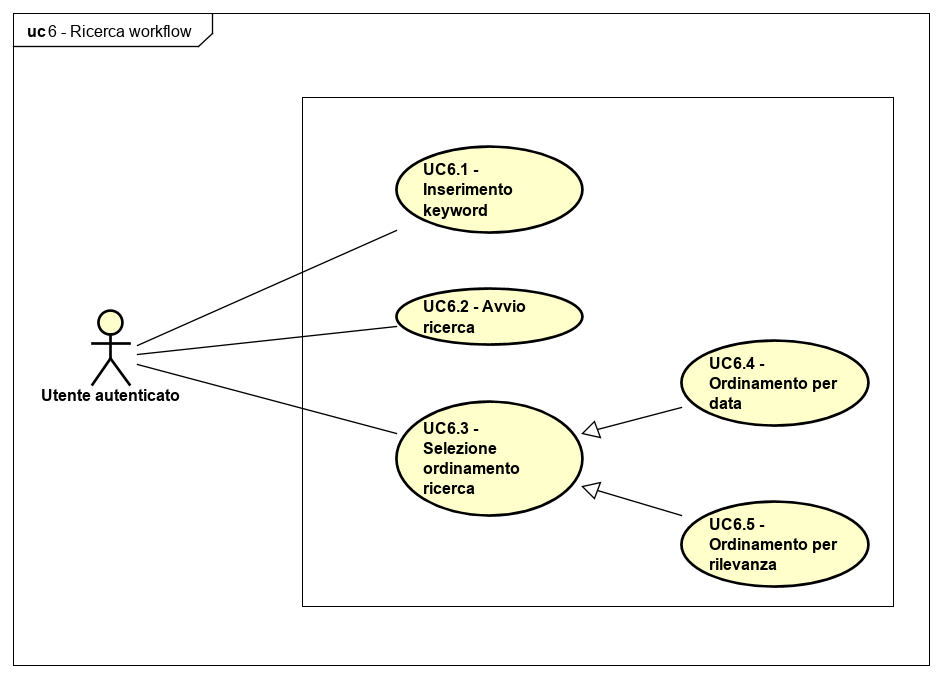
\includegraphics[scale=0.5]{immagini/UC6}
    \caption{UC6 - Ricerca workflow \label{fig:UC6}}
\end{figure}

\begin{itemize}
\item \textbf{Attori primari}: utente autenticato;

\item \textbf{Descrizione}: l'attore può cercare un workflow specifico tra quelli già esistenti;

\item \textbf{Pre-condizione}: l'attore vuole cercare un workflow specifico tramite nome;

\item \textbf{Post-condizione}: viene visualizzata la pagina dei risultati della ricerca;

\item \textbf{Scenario principale}:
\begin{enumerate}
\item l'utente può inserire la keyword per la ricerca (UC6.1);
\item l'utente può avviare la ricerca (UC6.2);
\item l'utente può selezionare il filtro per data di creazione (UC6.3).
\end{enumerate}
\end{itemize}

\subsubsection{UC6.1 - inserimento keyword}

\begin{itemize}
\item \textbf{Attori primari}: utente autenticato;

\item \textbf{Descrizione}:  l'attore può inserire la keyword che vuole cercare nella barra di ricerca;

\item \textbf{Pre-condizione}: l'attore vuole cercare un workflow tramite una keyword;

\item \textbf{Post-condizione}: la keyword per la ricerca è stata inserita;

\item \textbf{Scenario principale}:
\begin{enumerate}
\item l'utente può inserire una keyword nella barra di ricerca.
\end{enumerate}
\end{itemize}

\subsubsection{UC6.2 - Avvio ricerca}

\begin{itemize}
\item \textbf{Attori primari}: utente autenticato;

\item \textbf{Descrizione}:  l'attore può avviare la ricerca di un workflow;

\item \textbf{Pre-condizione}: l'attore vuole avviare la ricerca del workflow;

\item \textbf{Post-condizione}: l'attore ha avviato la ricerca;

\item \textbf{Scenario principale}:
\begin{enumerate}
\item l'utente può avviare la ricerca di un workflow.
\end{enumerate}
\end{itemize}

\subsubsection{UC6.3 - Selezione ordinamento ricerca}

\begin{itemize}
\item \textbf{Attori primari}: utente autenticato;

\item \textbf{Descrizione}:  l'attore può ordinare i risultati della ricerca;

\item \textbf{Pre-condizione}: l'attore vuole ordinare i risultati della ricerca;

\item \textbf{Post-condizione}: i risultati vengono ordinati secondo le volontà dell'attore;

\item \textbf{Scenario principale}:
\begin{enumerate}
\item l'utente può ordinare i risultati della ricerca.
\end{enumerate}

\item \textbf{Generalizzazioni}:
\begin{enumerate}
\item l'utente può ordinare i risultati per data di creazione (UC6.4);
\item l'utente può ordinare i risultati per rilevanza (UC6.5).
\end{enumerate}
\end{itemize}

\subsubsection{UC6.4 - Ordinamento per data}

\begin{itemize}
\item \textbf{Attori primari}: utente autenticato;

\item \textbf{Descrizione}:  l'attore può ordinare i risultati della ricerca per data di creazione;

\item \textbf{Pre-condizione}: l'attore vuole ordinare i risultati della ricerca per data di creazione;

\item \textbf{Post-condizione}: i risultati vengono ordinati secondo le volontà dell'attore;

\item \textbf{Scenario principale}:
\begin{enumerate}
\item l'utente può ordinare i risultati per data di creazione.
\end{enumerate}
\end{itemize}

\subsubsection{UC6.5 - Ordinamento per rilevanza}

\begin{itemize}
\item \textbf{Attori primari}: utente autenticato;

\item \textbf{Descrizione}:  l'attore può ordinare i risultati della ricerca per rilevanza;

\item \textbf{Pre-condizione}: l'attore vuole ordinare i risultati della ricerca per rilevanza;

\item \textbf{Post-condizione}: i risultati vengono ordinati secondo le volontà dell'attore;

\item \textbf{Scenario principale}:
\begin{enumerate}
\item l'utente può ordinare i risultati per rilevanza.
\end{enumerate}
\end{itemize}

\subsection{UC7 - Visualizzazione workflow}

\begin{itemize}
\item \textbf{Attori primari}: utente autenticato;

\item \textbf{Descrizione}:  l'attore può visualizzare i workflow precedentemente creati;

\item \textbf{Pre-condizione}: l'attore vuole visualizzare i propri workflow creati;

\item \textbf{Post-condizione}: Vengono visualizzati tutti i workflow creati dall'attore;

\item \textbf{Scenario principale}:
\begin{enumerate}
\item l'utente può visualizzare tutti i workflow creati.
\end{enumerate}
\end{itemize}

\subsection{UC8 - Logout}

\begin{itemize}
\item \textbf{Attori primari}: utente autenticato;

\item \textbf{Descrizione}: l'attore può eseguire l'operazione di logout;

\item \textbf{Pre-condizione}: l'utente è autenticato all'interno del sistema;

\item \textbf{Post-condizione}: l'utente non è più autenticato all'interno del sistema;

\item \textbf{Scenario principale}:
\begin{enumerate}
\item l'utente può effettuare l'operazione di logout.
\end{enumerate}
\end{itemize}
